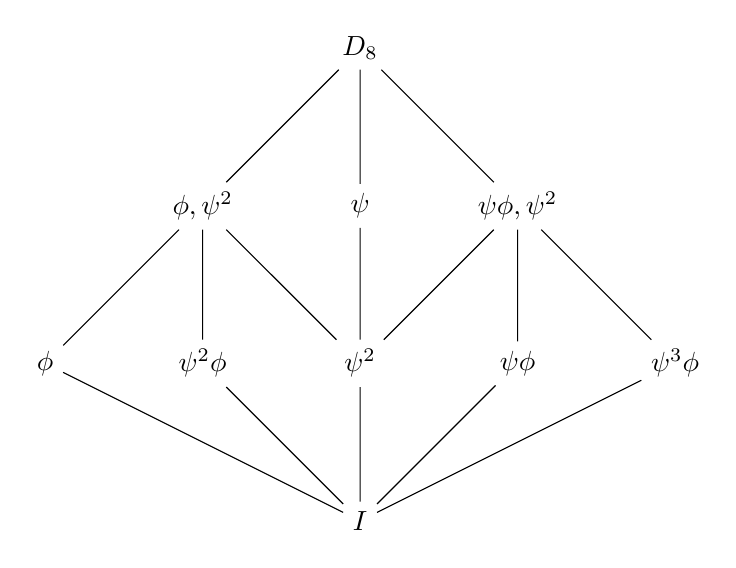
\begin{tikzpicture}[node distance=2cm]
    \node(D8) {$D_8$};
    \node(r)   [below of=D8] {$\angleBracket{\psi}$};
    \node(sr2) [left of= r] {$\angleBracket{\phi,\psi^2}$};
    \node(rsr2) [right of=r]{$\angleBracket{\psi \phi,\psi^2}$};
    \node(r2)[below of=r] {$\angleBracket{\psi^2}$};
    
    \node(r2s) [left of=r2]{$\angleBracket{\psi^2 \phi}$};
    \node(s) [left of=r2s] {$\angleBracket{\phi}$};

    \node(rs)[right of=r2] {$\angleBracket{\psi \phi}$};
    \node(r3s)[right of= rs] {$\angleBracket{\psi^3 \phi}$};
    \node(i)            [below of=r2]     {$\angleBracket{I}$};


    \draw (D8) -- (sr2)
    (D8) -- (r)
    (D8) -- (rsr2)
    (sr2) -- (s)
    (sr2) -- (r2s)
    (sr2) -- (r2)
    (r) -- (r2)
    (rsr2) -- (r2)
    (rsr2) -- (rs)
    (rsr2) -- (r3s)
    (s) -- (i)
    (r2s) -- (i)
    (r2) -- (i)
    (rs) -- (i)
    (r3s) -- (i);
\end{tikzpicture}
